\begin{frame}{Triangle construction}
\begin{enumerate}
\conti
\item In $\triangle{ABC}$ ,a=8,$\angle{B}=45\degree$ and c-b=3.5. Sketch $\triangle{ABC}$
\seti
\end{enumerate}
\textbf{Solution:}
\begin{figure}[!ht]
\resizebox{1\linewidth}{!}
{
\begin{tikzpicture}[scale =1,>=stealth,point/.style = {draw, circle, fill = black, inner sep = 2pt},]
\node (A) at (8.482904196010466,8.482904196010463)[point,label=above :$A$] {};
\node (B) at (0,0)[point,label=above :$B$] {};
\node (C) at (8,0)[point,label=below :$C$] {};
\draw[->,thick] (A) -- node[above] {$\textbf{c}$} (B) -- node[left] {$\textbf{a=8cm}$} (C) -- node[below,,xshift=1mm] {$\textbf{b}$} (A);
%Drawing and marking angles
\tkzMarkAngle[fill=white!45,size=.3,mark=](C,B,A)
\tkzLabelAngle[pos=0.65](A,B,C){$45$}
\end{tikzpicture}

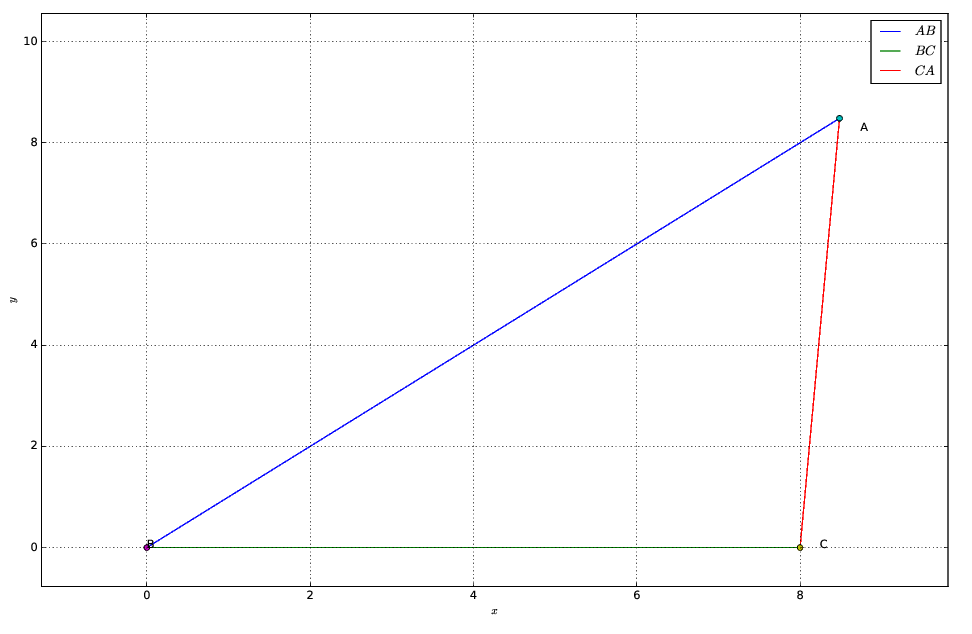
\includegraphics[scale=0.4]{./figs/triangle/constr.png}
}
\caption{Triangle with tikz and python }
\label{fig:foo}
\end{figure}
\end{frame}
\begin{frame}
Given a=8cm, c-b=k (k=3.5cm)
Apply cosine rule 
\begin{align*}
	\cos{(B)} = \frac{a^2+c^2-b^2}{2ac}\\
	\cos{(B)}= \frac{a^2+(b+k)^2-b^2}{2a(b+k)}\\
	2ab\cos{B}+2ak\cos{B}=a^2+k+2bk\\
	b=\frac{a^2 + k^2-2ak \cos{B} }{2a\cos{B}-2k}
\end{align*}
\begin{center}
b=8.49, c=11.99
\end{center}
\begin{itemize}
\item tikz code for above figure: \url{https://github.com/d-DP/Assignments/blob/master/figs/2.tex}
\item Python code for Figure 0-2:\url{https://github.com/d-DP/Assignments/blob/master/codes/2.py}\\
\end{itemize}
\end{frame}